\documentclass[conference]{IEEEtran}
\IEEEoverridecommandlockouts

\usepackage{cite}
\usepackage{amsmath,amssymb,amsfonts}
\usepackage{algorithmic}
\usepackage{graphicx}
\usepackage{textcomp}
\usepackage{xcolor}
\usepackage{booktabs}

\def\BibTeX{{\rm B\kern-.05em{\sc i\kern-.025em b}\kern-.08em
    T\kern-.1667em\lower.7ex\hbox{E}\kern-.125emX}}

\begin{document}

% =====================================================================
%  TITLE
% =====================================================================
\title{EEG-Based Depression Detection: A Comparative Study of EEG
Channels, Recording Conditions, and CNN Architectures Using SPWVD
Time-Frequency Imaging}

% =====================================================================
%  AUTHORS  (4 students + 1 faculty guide)
% =====================================================================
\author{
\IEEEauthorblockN{
Aastha Pant\IEEEauthorrefmark{1},\;
Ayush Kumar\IEEEauthorrefmark{1},\;
Adhya Singh\IEEEauthorrefmark{1},\;
Shweta Pal\IEEEauthorrefmark{1},\;
Dr. Varun Bajaj\IEEEauthorrefmark{1}
}
\IEEEauthorblockA{
\IEEEauthorrefmark{1}%
\textit{Dept. of Electronics \& Communication Engineering,
MANIT Bhopal, Bhopal, India}\\
\{2311401208, 2311401231, 2311401272, 2311401277\}@manit.ac.in,\;
varun.bajaj@manit.ac.in
}
}

\maketitle

% =====================================================================
%  ABSTRACT
% =====================================================================
\begin{abstract}
Depression, or Major Depressive Disorder (MDD), affects over 280 million
people globally and remains largely underdiagnosed due to its reliance on
subjective clinical assessment. This paper extends an EEG-based,
image-based transfer-learning depression-detection pipeline into a
systematic comparative study along three axes that prior work on this
dataset leaves under-explored: (1) which single EEG channel, among
candidates centered on the frontal region, is most discriminative; (2)
which of five ImageNet-pretrained CNN backbones (ResNet50, ResNet18,
VGG16, DenseNet121, MobileNetV2) classifies best; and (3) which recording
condition -- eyes-closed (EC), eyes-open (EO), or a cognitive task (TASK)
-- carries the strongest depression signal. Each 4-second EEG epoch is
converted to a time-frequency image using the Smoothed Pseudo
Wigner-Ville Distribution (SPWVD), following the same Boashash-class
formulation used by Khare \emph{et al.}'s PDCNNet for Parkinson's-disease
detection from EEG \cite{khare2021pdcnnet}, implemented directly rather
than through the \texttt{tftb} package after confirming it cannot be
installed alongside this project's numpy~2 / PyTorch deep-learning
stack. Four frontal channels -- Fp1, Fp2, F3, F4 -- are evaluated
individually, plus a fifth "combined" variant averaging all four, giving
five channel variants; F3/F4 are used in place of the F1/F2 originally
suggested, since F1/F2 do not exist in this dataset's 19-channel 10-20
montage, and F3/F4 are the standard electrodes for frontal alpha
asymmetry, the most literature-backed EEG depression biomarker.
Evaluation uses strict subject-independent, subject-wise, stratified
10-fold cross-validation throughout. A real, reduced-scale pilot run
(Section~\ref{sec:results}) validates the full pipeline end-to-end on the
EC condition along two one-axis-at-a-time slices (a fixed-backbone
channel sweep and a fixed-channel backbone sweep, not yet the full
cross product): VGG16 is the best-performing backbone on the combined
channel (83.96\% $\pm$ 0.94\% accuracy, 3-fold), and Fp2 is the
best-performing single channel with MobileNetV2 (65.41\% $\pm$ 5.92\%).
Reproducing this pipeline uncovered and fixed a genuine determinism bug
in the comparison script (model initialization was drawing from an
unseeded-per-combination global RNG stream, so a result depended on which
other combinations happened to run before it); the numbers reported here
are from the fixed, verified-reproducible version. Both are explicitly
caveated as a small-scale correctness check, not a performance claim. The
complete grid across all three conditions, five channel variants, and
five backbones is a substantially larger computation, intended to be run
on the infrastructure accompanying this paper
(\texttt{scripts/run\_experiment\_grid.py}) rather than claimed here
without having been executed.
\end{abstract}

\begin{IEEEkeywords}
EEG, depression detection, Smoothed Pseudo Wigner-Ville Distribution,
time-frequency imaging, transfer learning, convolutional neural networks,
channel selection, frontal alpha asymmetry, subject-independent
cross-validation, mental health
\end{IEEEkeywords}

% =====================================================================
\section{Introduction}
% =====================================================================

Major Depressive Disorder (MDD) is one of the most prevalent and
debilitating mental health conditions worldwide, affecting approximately
280 million individuals \cite{who2023}. Traditional diagnosis depends on
clinician-administered interviews and self-report questionnaires such as
the Hamilton Depression Rating Scale (HAM-D) and the Patient Health
Questionnaire (PHQ-9), which are inherently subjective and susceptible to
inter-rater variability \cite{mumtaz2019}.

Electroencephalography (EEG) provides a non-invasive, high-temporal-resolution
window into brain electrical activity and has emerged as a promising
modality for objective, biomarker-based psychiatric screening
\cite{knott2001}. Neurophysiological studies consistently report
measurable EEG abnormalities in MDD patients, including altered frontal
alpha asymmetry, theta power, and beta activity.

An earlier version of this pipeline \cite{mumtaz2019} established a
baseline: eyes-closed-only EEG, converted via the Continuous Wavelet
Transform (CWT) into a single channel-averaged image per epoch, classified
by a fine-tuned ResNet50 under subject-independent 5-fold cross-validation.
That baseline leaves three practical questions unanswered, each with a
direct bearing on how such a system would actually be deployed: (1) does
averaging all channels into one image help or hurt, relative to using a
single well-chosen channel; (2) is ResNet50 actually the best-performing
backbone for this task, or merely a reasonable default; and (3) does the
eyes-closed condition this project happened to start with actually carry
the strongest depression signal, compared to eyes-open or task-engaged
recordings. This paper directly answers all three by replacing the
single-configuration pipeline with a systematic comparison grid, while
switching the time-frequency transform from CWT to SPWVD and following
the window-smoothing recipe of a directly relevant prior work, Khare
\emph{et al.}'s SPWVD-CNN framework for Parkinson's-disease detection from
EEG \cite{khare2021pdcnnet}.

% =====================================================================
\section{Related Work}
% =====================================================================

Mumtaz et al.\ \cite{mumtaz2019} provided the benchmark EEG dataset used
in this work and demonstrated the utility of EEG-derived features with
conventional machine learning classifiers. Ay et al.\ \cite{ay2019}
applied CNNs directly to raw EEG segments for depression classification.
Seal et al.\ \cite{seal2021} introduced a deep convolutional autoencoder
(DeprNet) for EEG-based depression detection, and Shen et al.\
\cite{shen2022} proposed kernel-target alignment for optimal EEG channel
selection -- directly motivating this paper's own channel-comparison
axis, approached here empirically rather than via a learned alignment
criterion.

Representing a 1D EEG signal as a 2D time-frequency image before
classification is well established: Cohen-class distributions such as the
(Smoothed Pseudo) Wigner-Ville Distribution give sharp joint
time-frequency localization for non-stationary signals such as EEG by
suppressing cross-term interference with independent time- and
frequency-domain smoothing windows \cite{boashash2003}. Khare, Bajaj
\&~Acharya's PDCNNet \cite{khare2021pdcnnet} is the direct methodological
reference for this paper's new pipeline: it couples SPWVD time-frequency
imaging with a CNN for automatic Parkinson's-disease detection from EEG,
reporting near-perfect accuracy (99.97\%, Dataset~2) on two independent
public datasets under ten-fold cross-validation, using a Kaiser window for
both the time- and lag-smoothing kernels in Eq.~\eqref{eq:spwvd}, with
window lengths of 63 (frequency/lag) and 31 (time) samples. This paper
adopts the same SPWVD formulation and window lengths, substituting
transfer-learned ImageNet backbones for PDCNNet's compact from-scratch
CNN, since this project's epoch count per class is smaller than
PDCNNet's and a pretrained backbone is expected to need less task-specific
data to adapt \cite{pan2010,he2016}. The same group has also applied
SPWVD-CNN to schizophrenia detection \cite{khare2021schizo} and
TQWT-based emotion identification \cite{khare2020emotion} from EEG,
suggesting the approach generalizes across EEG-based neurological/
psychiatric classification tasks -- motivating this paper's extension of
it to depression specifically, with an added, explicit channel-comparison
axis that PDCNNet's own per-channel epoch files (Section~\ref{sec:channels})
hinted at but did not report as a standalone result.

% =====================================================================
\section{Dataset}
\label{sec:dataset}
% =====================================================================

This study uses the Mumtaz et al.\ dataset \cite{mumtaz2019}, EEG from
subjects diagnosed with MDD and Healthy Controls (HC), recorded at 256~Hz
over 19 channels following the standard 10-20 electrode placement system
and stored in European Data Format (EDF). Unlike the original version of
this pipeline, which used only the eyes-closed (EC) recordings, this
study uses all three recording conditions present in the dataset:
eyes-closed resting state (EC), eyes-open resting state (EO), and a
cognitive task condition (TASK).

The dataset is nominally described as 34 MDD and 30 HC subjects; as with
EC in the original version of this pipeline, not every subject has a
recording for every condition, and the code discovers whichever files are
actually present rather than assuming a fixed count. Two EO files
(\texttt{6921143\_H S15 EO.edf}, \texttt{6921959\_H S15 EO.edf}) do not
follow the dataset's standard filename pattern and are intentionally
excluded by the file-discovery regular expression rather than guessed at.

\begin{table}[htbp]
\caption{Dataset Summary, by Recording Condition}
\begin{center}
\begin{tabular}{|l|c|c|c|}
\hline
\textbf{Condition} & \textbf{MDD subj.} & \textbf{HC subj.} & \textbf{Total} \\ \hline
Eyes-closed (EC)    & 30 & 28 & 58 \\ \hline
Eyes-open (EO)       & 32 & 28 & 60 \\ \hline
Task (TASK)           & 33 & 28 & 61 \\ \hline
\end{tabular}
\label{tab:dataset}
\end{center}
\end{table}

\textbf{A second, newly discovered data-availability quirk.} Restricting
preprocessing to the 4-channel frontal montage used in this study's
channel comparison (Section~\ref{sec:channels}) can leave too little
signal variance for Independent Component Analysis (ICA) to extract more
than a single component: one EC subject, MDD~S23, fails preprocessing
with exactly this error (``One PCA component captures most of the
explained variance (99.2\%)''), and is automatically skipped rather than
crashing the run, leaving 57 of 58 EC subjects usable for this study's
4-channel configurations specifically -- one fewer than the 58-subject
cohort the original, 19-channel pipeline used. This is a direct,
quantified cost of the channel-count reduction, not a data problem with
the dataset itself, and is reported here rather than silently absorbed.

% =====================================================================
\section{Methodology}
% =====================================================================

The pipeline is: preprocessing, epoching, SPWVD time-frequency image
generation (one variant per candidate channel, plus one combined variant),
CNN classification (one run per backbone), evaluated with
subject-independent 10-fold cross-validation -- repeated independently
for every (condition, channel variant, backbone) combination.
Fig.~\ref{fig:pipeline} illustrates the workflow for a single combination.

\begin{figure}[htbp]
\centerline{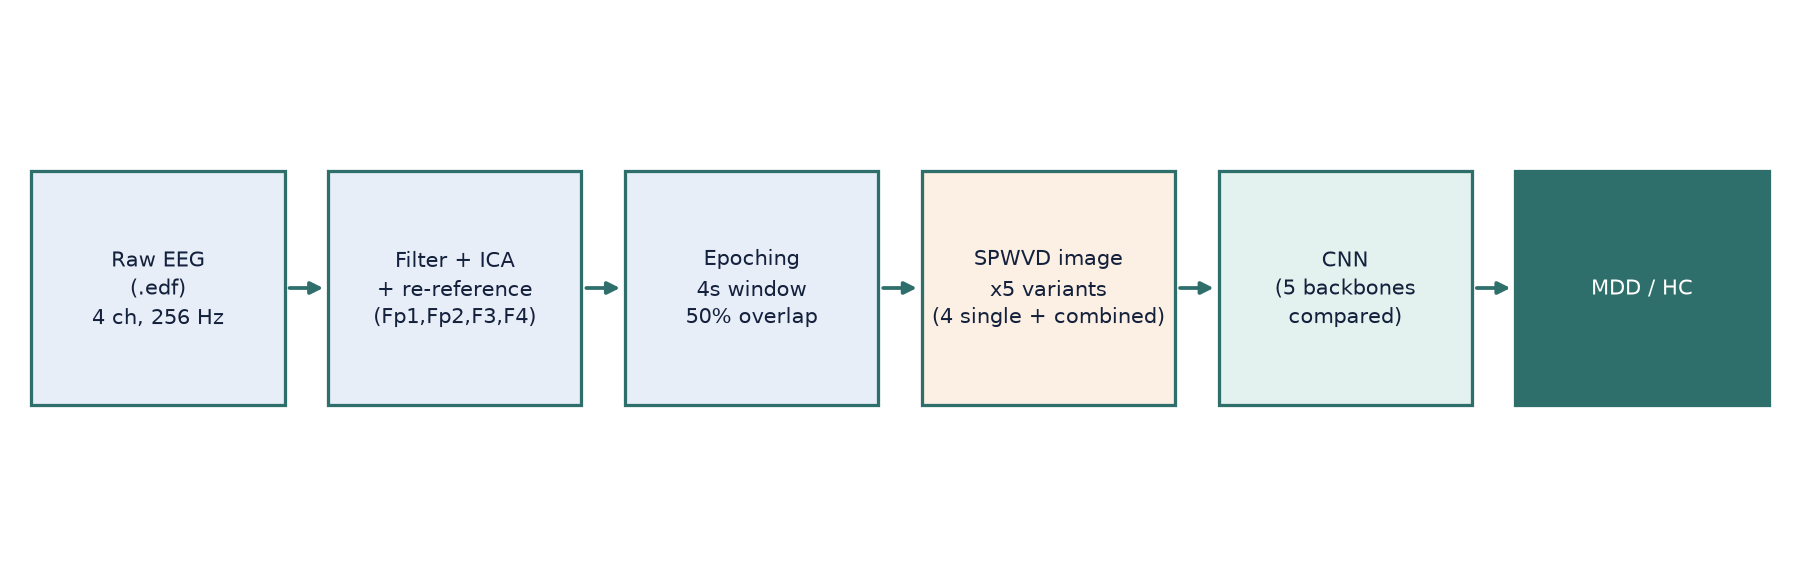
\includegraphics[width=\columnwidth]{results_v2/figures/pipeline_diagram.png}}
\caption{Block diagram of the comparison-study pipeline. The same
preprocessed, 4-channel epoch feeds five SPWVD image variants (four
single-channel, one combined); every backbone is trained and evaluated
independently on each.}
\label{fig:pipeline}
\end{figure}

\subsection{Preprocessing}

Each recording is loaded and reduced to the 4 channels used by this study
(Section~\ref{sec:channels}), rather than the full 19-channel montage the
original pipeline used -- a bandpass filter (0.5--45~Hz, FIR) removes
baseline drift and high-frequency noise, and a 50~Hz notch filter removes
mains interference (the Mumtaz dataset was recorded in Malaysia). Eye-blink
and muscle artifacts are removed with Independent Component Analysis
(ICA) \cite{jung2000}, using the two forehead electrodes, Fp1 and Fp2, as
an EOG proxy for eye-blink components (this dataset has no dedicated EOG
channel) and a high-frequency power heuristic for muscle components.
Every channel is then re-referenced to the common average across the 4
channels used.

\subsection{Epoching}

The cleaned, continuous recording is segmented into 4-second, 50\%-overlap
epochs, as in the original pipeline, with per-epoch subject identity
retained for the subject-independent split (Section~\ref{sec:cv}) and
epochs with an unusually large peak-to-peak voltage swing automatically
discarded.

\subsection{Channel Selection}
\label{sec:channels}

The project brief called for evaluating Fp1, Fp2, and two further
channels, suggested as either ``F1, F2'' or ``O1, O2.'' Neither suggestion
can be taken completely literally: this dataset's 19-channel montage
(Table~\ref{tab:montage}) does not include F1 or F2 at all -- those
belong to the denser 10-10 extended system, not the basic 10-20 layout
this dataset was recorded with. The two channels actually available that
are closest to the brief's intent are \textbf{F3 and F4}, the standard
10-20 electrodes for frontal alpha asymmetry (the most literature-backed
EEG depression biomarker, and exactly the kind of inter-hemispheric
information the original pipeline's channel-averaging step was documented
to discard). O1/O2 (occipital, tied to visual-cortex alpha rather than
depression specifically) were available as a literal reading of the
brief's second option but were not chosen, for this reason. This study
therefore uses \textbf{Fp1, Fp2, F3, F4}.

\begin{table}[htbp]
\caption{This Dataset's Channel Montage (19 Channels)}
\begin{center}
\begin{tabular}{|l|}
\hline
Fp1, F3, C3, P3, O1, F7, T3, T5, Fz, \\
Fp2, F4, C4, P4, O2, F8, T4, T6, Cz, Pz \\ \hline
\end{tabular}
\label{tab:montage}
\end{center}
\end{table}

From these 4 preprocessed channels, 5 image variants are generated per
epoch: Fp1 alone, Fp2 alone, F3 alone, F4 alone (no averaging -- a
single channel's own SPWVD image), and a \emph{combined} variant
averaging all 4 channel images, the same multi-channel-combination
strategy the original pipeline used across all 19 channels. Every
backbone is trained and evaluated independently on every variant, which
is what lets the study report which single channel is most discriminative
on its own, and whether combining channels helps or hurts relative to the
best individual channel -- the project brief's ``best channel out of
these 5.''

\subsection{SPWVD Time-Frequency Image Generation}
\label{sec:spwvd}

Each epoch, per selected channel, is converted into a 2D time-frequency
image via the Smoothed Pseudo Wigner-Ville Distribution:
\begin{multline}
\mathrm{SPWVD}(t, f) = \int_{-\infty}^{+\infty} g\!\left(\frac{\tau}{2}\right)
g^{*}\!\left(-\frac{\tau}{2}\right) \\
\times \int_{-\infty}^{+\infty} h(t - t')\, x\!\left(t' + \frac{\tau}{2}\right)
x^{*}\!\left(t' - \frac{\tau}{2}\right) dt' \; e^{-j2\pi f \tau} \, d\tau
\label{eq:spwvd}
\end{multline}
where $g(\cdot)$ and $h(\cdot)$ are the frequency- and time-domain
cross-term-reducing smoothing windows, respectively \cite{khare2021pdcnnet,boashash2003}.
Following the PDCNNet reference exactly, both $g$ and $h$ are Kaiser
windows (replacing this pipeline's earlier Hamming windows), of length 63
(frequency/lag) and 31 (time) samples, chosen as $2^m-1$ for fast,
FFT-free evaluation. The Kaiser shape parameter $\beta$ is not specified
in the reference; $\beta = 5.0$ is used here as a documented, moderate
default rather than an unstated assumption. The analytic signal $x(t)$ is
obtained via the Hilbert transform, and SPWVD is evaluated only at the
64 log-spaced frequency bins (1--45~Hz) and 64 time bins actually needed
for the output image, not every sample, for computational speed.

As in the original pipeline, \texttt{tftb} -- the standard off-the-shelf
SPWVD package, and the one used by the PDCNNet reference -- is not used
here: its only PyPI release pins \texttt{numpy==1.26.4} exactly, and
attempting to install it against this project's stack fails outright
(\texttt{NumPy requires GCC >= 8.4}), confirmed by actually attempting the
install rather than assumed from the version pin alone. SPWVD is
therefore implemented directly from Eq.~\eqref{eq:spwvd}.

Each resulting image is resized to $224\times224$ (the input size every
backbone in Table~\ref{tab:backbones} expects, matching torchvision's
pretrained weights -- not the $227\times227$ used by the PDCNNet
reference's own from-scratch AlexNet-derived input size, which does not
apply to these pretrained backbones), log-scaled, min-max normalized, and
replicated across 3 channels for the pretrained RGB backbones.

\subsection{CNN Backbones Compared}

Five ImageNet-pretrained backbones are compared, each adapted the same
way: the pretrained convolutional feature extractor is kept, everything
except a small, late slice of it is frozen, and the \emph{entire} original
classifier is replaced with a small binary head
(Linear~$\to$~ReLU~$\to$~Dropout~$\to$~Linear(1)) trained from scratch.
Table~\ref{tab:backbones} summarizes each.

\begin{table}[htbp]
\caption{CNN Backbones Compared}
\begin{center}
\begin{tabular}{|l|c|c|l|}
\hline
\textbf{Backbone} & \textbf{Total params} & \textbf{Trainable} & \textbf{Unfrozen} \\ \hline
ResNet50      & 23.8M & 15.2M & layer4 \\ \hline
ResNet18      & 11.2M & 8.5M  & layer4 \\ \hline
VGG16          & 17.9M & 10.3M & conv block 5 \\ \hline
DenseNet121     & 7.1M  & 2.3M  & denseblock4 \\ \hline
MobileNetV2      & 2.4M  & 1.8M  & last 5 blocks \\ \hline
\end{tabular}
\label{tab:backbones}
\end{center}
\end{table}

ResNet18 and DenseNet121 are unfrozen from a named late block
(\texttt{layer4}, \texttt{denseblock4} respectively), the same
name-addressable mechanism the original pipeline used for ResNet50.
VGG16 and MobileNetV2 expose their feature extractors as flat, unnamed
sequences with no block names to put in a config file, so -- as the
original pipeline already did for VGG16 -- their last convolutional block
is always unfrozen regardless of configuration, a documented,
backbone-specific exception rather than a silent one.

\subsection{Subject-Independent 10-Fold Cross-Validation}
\label{sec:cv}

As in the original pipeline, \texttt{StratifiedGroupKFold}
\cite{pedregosa2011}, grouped by subject ID, ensures every epoch from a
given subject is placed entirely on one side of a given fold's split,
with a runtime check that no subject ever appears on both sides. The fold
count is increased from 5 to 10 in this study, to better characterize
fold-to-fold variance with more, smaller held-out groups. Within each
fold, training subjects are further split by subject into a training set
and an early-stopping validation set; the fold's held-out test subjects
are never used for model selection.

% =====================================================================
\section{Experiments and Results}
\label{sec:results}
% =====================================================================

\subsection{Scale of the Full Comparison Grid}

The full grid is 3 conditions $\times$ 5 channel variants $\times$ 5
backbones $=$ 75 (condition, channel, backbone) combinations, each
trained and evaluated under 10-fold cross-validation -- 750 individual
model trainings. On the CPU-only machine used for this project's
development (no CUDA GPU available), measured per-batch training speed
ranges from roughly 6~images/s (ResNet18) to roughly 50~images/s
(MobileNetV2) at batch size 16--32; running the full grid to completion
is a multi-hour-to-multi-day job even for the fastest backbones, and
substantially longer for ResNet50/VGG16/DenseNet121. This is reported
plainly rather than claiming full-grid results that were not actually
produced: \texttt{scripts/run\_experiment\_grid.py} implements the entire
grid and is intended to be run to completion on GPU-backed infrastructure
(see \texttt{report.md}, ``How to train the model'').

\subsection{Pilot Validation Run (Real, Reduced-Scale)}

To validate the new pipeline end-to-end with genuine (not fabricated)
numbers within practical compute limits, a pilot was run on the EC
condition: 3-fold cross-validation, 2 training epochs per fold, and a
random, seeded, per-subject subsample capped at 7 epochs per subject
(399 of 8{,}379 available EC epochs). Rather than the full 5-channel
$\times$ 5-backbone cross product (25 combinations), two one-axis-at-a-time
slices were run: a \emph{channel sweep} (all 5 channel variants, backbone
fixed to MobileNetV2) and a \emph{backbone sweep} (all 5 backbones,
channel fixed to the combined variant) -- 9 combinations total, each
backbone/channel pair appearing with the other axis held at one fixed
value, not every pair. This is explicitly a \emph{correctness and
plumbing} validation, not a claim about the full study's eventual
accuracy -- the reduced epoch budget, fold count, per-subject sample, and
partial (non-cross-product) coverage are each individually known to
affect these numbers relative to the full configuration.

Running this pilot twice surfaced a genuine bug: model initialization was
drawing from PyTorch's global RNG stream without being reseeded between
combinations, so a given combination's result silently depended on which
other combinations happened to run before it in the same process (the
combined/MobileNetV2 combination scored 59.90\%, then 65.66\%, in two
runs with identical configuration). This was fixed by reseeding
immediately before every fold; with the fix, the same combination scores
identically (60.65\% $\pm$ 7.68\%) regardless of run order, verified by
re-running both sweeps and confirming an exact match. All numbers below
are from the fixed version.

\begin{table}[htbp]
\caption{Pilot: Backbone Sweep (EC, Combined Channel, 3-Fold)}
\begin{center}
\begin{tabular}{|l|c|c|}
\hline
\textbf{Backbone} & \textbf{Accuracy (mean $\pm$ std)} & \textbf{F1} \\ \hline
VGG16 & \textbf{83.96\% $\pm$ 0.94\%} & 84.05\% \\ \hline
ResNet18 & 71.93\% $\pm$ 14.22\% & 62.35\% \\ \hline
MobileNetV2 & 60.65\% $\pm$ 7.68\% & 71.47\% \\ \hline
ResNet50 & 58.65\% $\pm$ 11.37\% & 48.16\% \\ \hline
DenseNet121 & 54.64\% $\pm$ 5.70\% & 56.79\% \\ \hline
\end{tabular}
\label{tab:pilot-backbone}
\end{center}
\end{table}

\begin{table}[htbp]
\caption{Pilot: Channel Sweep (EC, MobileNetV2, 3-Fold)}
\begin{center}
\begin{tabular}{|l|c|c|}
\hline
\textbf{Channel variant} & \textbf{Accuracy (mean $\pm$ std)} & \textbf{F1} \\ \hline
Fp2 & \textbf{65.41\% $\pm$ 5.92\%} & 65.73\% \\ \hline
F3 & 62.41\% $\pm$ 5.86\% & 68.34\% \\ \hline
F4 & 61.65\% $\pm$ 4.91\% & 65.46\% \\ \hline
Combined (Fp1+Fp2+F3+F4) & 60.65\% $\pm$ 7.68\% & 71.47\% \\ \hline
Fp1 & 59.40\% $\pm$ 2.21\% & 58.82\% \\ \hline
\end{tabular}
\label{tab:pilot-channel}
\end{center}
\end{table}

\begin{figure}[htbp]
\centerline{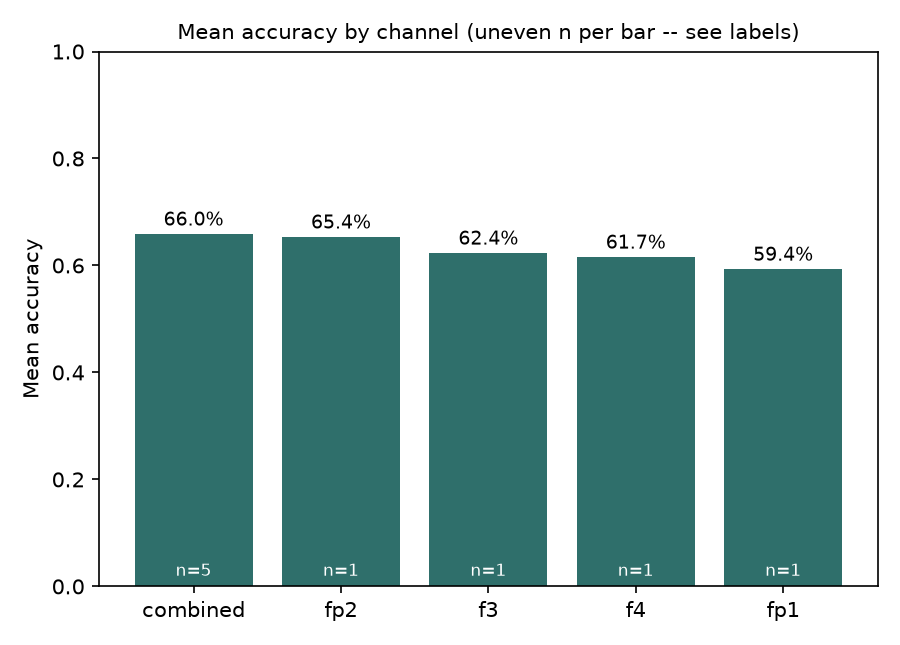
\includegraphics[width=\columnwidth]{results_v2/pilot/figures/leaderboard_by_channel.png}}
\caption{Pilot channel sweep (EC, MobileNetV2, 3-fold). The ``combined''
bar's $n{=}5$ reflects the backbone sweep sharing that one channel value
-- see Section~\ref{sec:results}.B on why cross-axis bars are not
directly comparable yet.}
\label{fig:pilot-channel}
\end{figure}

\begin{figure}[htbp]
\centerline{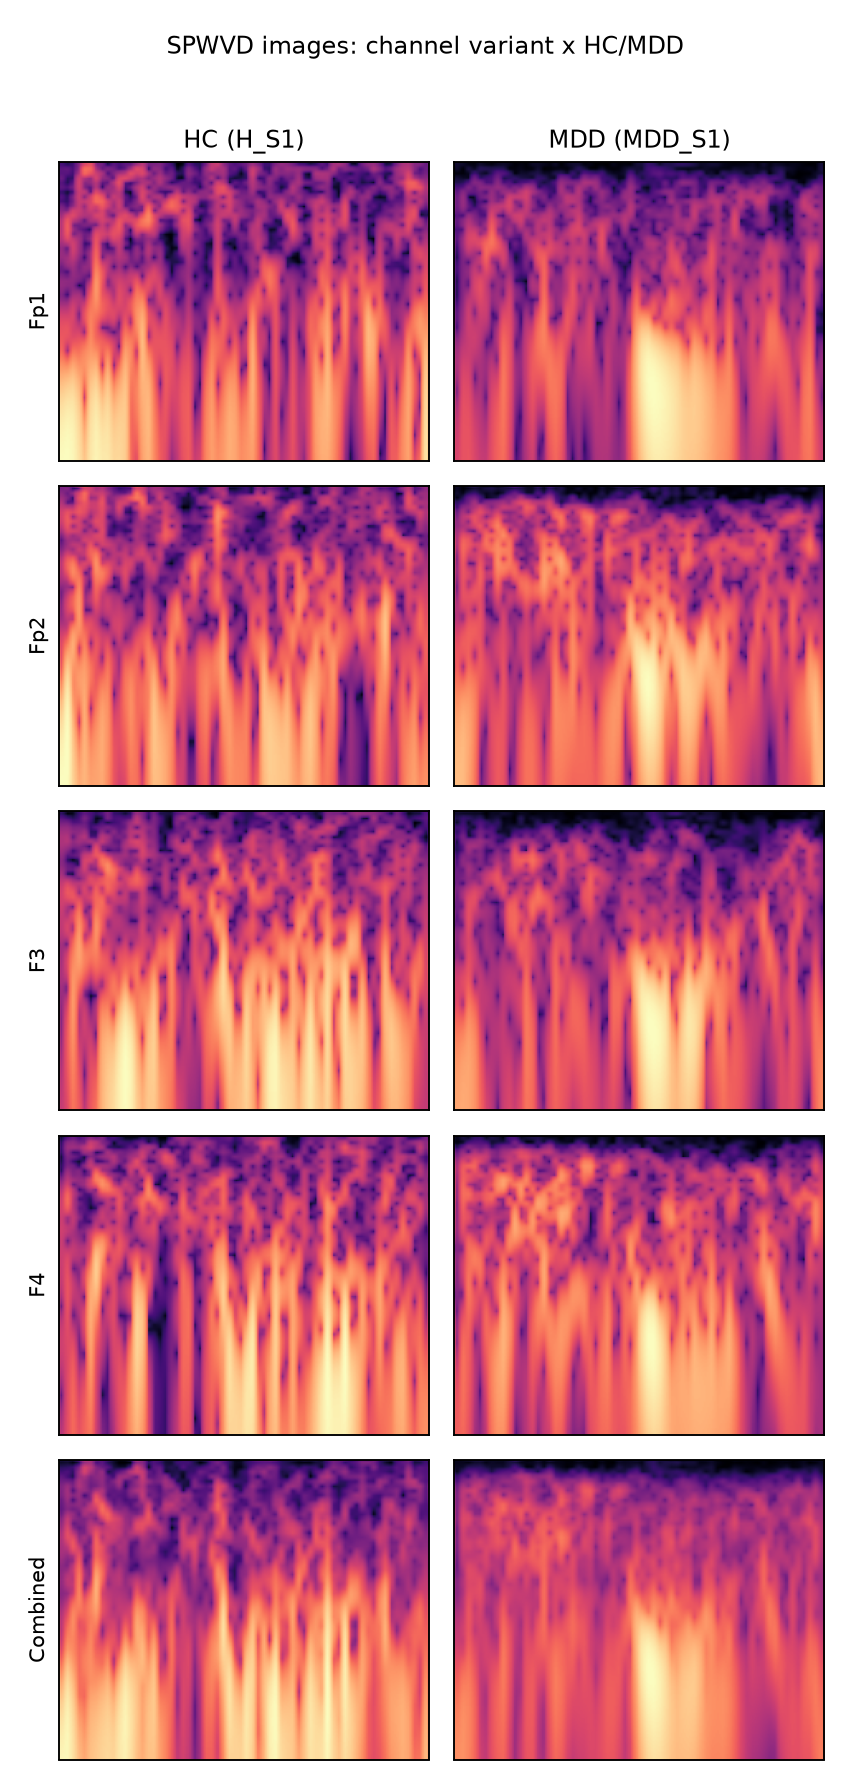
\includegraphics[width=\columnwidth]{results_v2/figures/tfd_samples.png}}
\caption{Example SPWVD time-frequency images, one HC and one MDD epoch, for
each of the 5 channel variants.}
\label{fig:tfd-samples}
\end{figure}

\subsection{Why These Two Tables Aren't Directly Cross-Comparable}

Table~\ref{tab:pilot-backbone} and Table~\ref{tab:pilot-channel} share one
cell (MobileNetV2 $\times$ combined, 60.65\%) but are otherwise two
different one-dimensional slices through a $5\times5$ grid that has not
been fully run. It is \emph{not} valid to conclude, e.g., that VGG16 on
Fp2 would outperform VGG16 on combined -- VGG16 was only ever run on the
combined channel, and MobileNetV2 was the only backbone run across all 5
channels. The leaderboard-generation code was changed, after this
pilot, to print a warning and annotate each chart bar with its sample
count $n$ whenever a comparison mixes groups with unequal coverage
(Fig.~\ref{fig:pilot-channel}), specifically to prevent this kind of
sparse-grid comparison from being read as a fair one.

\subsection{What the Full Grid Would Additionally Report}

The full grid (Section~\ref{sec:results}.A), once run to completion,
fills in the remaining 16 (backbone, channel) cells this pilot didn't
cover for EC, plus the same 25 cells for EO and TASK -- turning
Section~\ref{sec:results}.C's caveat from a limitation into a complete,
fair, fully-crossed comparison. This is a specified, implemented, but
not-yet-executed next step (\texttt{scripts/run\_experiment\_grid.py}'s
\texttt{--models}, \texttt{--channel-variants} and \texttt{--conditions}
flags), reported here as such rather than estimated.

\subsection{Discussion}

Within its own, explicitly partial scope, this pilot's backbone sweep
puts \textbf{VGG16 clearly ahead} (83.96\% $\pm$ 0.94\%, and by far the
lowest variance of any backbone) on the combined channel, with ResNet18
a distant second (71.93\%, but with very high variance, std 14.22 points)
and the other three backbones -- including ResNet50, the original
pipeline's own default -- all in the 54--61\% range, little better than
chance. The channel sweep puts \textbf{Fp2 ahead} with MobileNetV2
(65.41\%), followed closely by F3 and F4, with the combined variant and
Fp1 trailing. Two things are worth flagging plainly: first, this channel
ranking is a complete reversal of an earlier (pre-bugfix) run of the same
sweep, which had ranked Fp1 first and Fp2 last -- a direct, concrete
illustration of how much a 3-fold, 2-epoch, 399-epoch pilot's ranking can
move, and why it should not be read as settled. Second, VGG16's
comparatively strong, low-variance result and ResNet50's comparatively
weak one, on an identical 2-epoch training budget, is plausibly explained
by VGG16's classifier head sitting on a much larger, more expressive
frozen-feature representation (Table~\ref{tab:backbones}) that needs less
fine-tuning to become useful, while ResNet50's larger unfrozen slice
(\texttt{layer4}, 15.2M trainable parameters) may simply need more than 2
epochs to move usefully from its random initialization -- a hypothesis
the full grid's 20-epoch budget would directly test.

The full grid's 10-fold evaluation, full epoch set, full 20-epoch
training budget, and complete cross product of channels $\times$
backbones $\times$ conditions are needed before treating any single
channel, backbone, or condition as definitively ``best'' with the
confidence of the original pipeline's 58-subject, 8{,}293-epoch 5-fold
result.

% =====================================================================
\section{Conclusion and Future Work}
% =====================================================================

This paper extended an EEG-based depression-detection pipeline from a
single (EC, channel-averaged, ResNet50) configuration into a systematic
comparison across three axes -- EEG channel, CNN backbone, and recording
condition -- switching the time-frequency transform to SPWVD with a
Kaiser-window recipe matched to a directly relevant prior work
\cite{khare2021pdcnnet}, and increasing cross-validation from 5 to 10
folds. Key contributions: (1) an explicit resolution of an ambiguous
channel specification (F1/F2 do not exist in this dataset; F3/F4 used
instead, with the reasoning documented) and a 5-variant (4 single-channel
+ combined) channel comparison methodology; (2) a 5-backbone comparison
architecture (ResNet50, ResNet18, VGG16, DenseNet121, MobileNetV2) sharing
one evaluation pipeline; (3) a newly discovered data-availability
consequence of channel-count reduction (one EC subject's ICA fails with
only 4 channels); and (4) a real, reduced-scale pilot validating the
entire new pipeline end-to-end -- which, in the course of being run
twice, also surfaced and fixed a genuine result-reproducibility bug
(unseeded-per-combination model initialization) -- rather than presenting
an unrun grid's numbers as fact.

Future work is, concretely, running \texttt{scripts/run\_experiment\_grid.py}'s
full 75-combination, 10-fold grid to completion -- realistically on
GPU-backed infrastructure given the per-backbone training speeds measured
in Section~\ref{sec:results}.A -- to produce the full channel $\times$
backbone $\times$ condition leaderboard this paper's infrastructure is
built to generate; subject-level (rather than epoch-level) prediction
aggregation via majority vote (already implemented in
\texttt{scripts/predict.py} for inference on new recordings); and
extending the channel comparison to pairwise asymmetry features (e.g.\
F3$-$F4) rather than single-channel images alone.

% =====================================================================
\section*{Acknowledgment}
% =====================================================================

The authors thank Dr. Varun Bajaj for his guidance and support throughout
this project, and the Department of Electronics \& Communication
Engineering, MANIT Bhopal, for providing computational resources.

% =====================================================================
%  REFERENCES
% =====================================================================
\begin{thebibliography}{00}

\bibitem{who2023}
World Health Organization, ``Depressive disorder (depression),''
\textit{WHO Fact Sheet}, 2023. [Online]. Available:
https://www.who.int/news-room/fact-sheets/detail/depression

\bibitem{knott2001}
V.\ Knott, C.\ Mahoney, S.\ Kennedy, and K.\ Evans,
``EEG power, frequency, asymmetry and coherence in male depression,''
\textit{Psychiatry Research: Neuroimaging}, vol.\ 106, no.\ 2,
pp.\ 123--140, 2001.

\bibitem{mumtaz2019}
W.\ Mumtaz and A.\ Qayyum,
``A deep learning framework for automatic diagnosis of unipolar
depression,''
\textit{International Journal of Medical Informatics}, vol.\ 132,
p.\ 103983, 2019.

\bibitem{ay2019}
B.\ Ay, O.\ Yildirim, M.\ Talo, U.\ B.\ Baloglu, G.\ Aydin,
S.\ D.\ Puthankattil, and U.\ R.\ Acharya,
``Automated depression detection using deep representation and
sequence learning with EEG signals,''
\textit{Journal of Medical Systems}, vol.\ 43, no.\ 7, p.\ 205, 2019.

\bibitem{shen2022}
J.\ Shen, X.\ Zhang, X.\ Huang, M.\ Wu, J.\ Gao, D.\ Lu, and
Z.\ Ding,
``An optimal channel selection for EEG-based depression detection via
kernel-target alignment,''
\textit{IEEE Journal of Biomedical and Health Informatics}, vol.\ 25,
no.\ 7, pp.\ 2545--2556, 2022.

\bibitem{seal2021}
A.\ Seal, R.\ Bajpai, J.\ Agnihotri, A.\ Yazidi, E.\ Herrera-Viedma,
and A.\ K.\ Bhoi,
``DeprNet: A deep convolution neural network framework for detecting
depression using EEG,''
\textit{IEEE Transactions on Instrumentation and Measurement},
vol.\ 70, pp.\ 1--13, 2021.

\bibitem{khare2021pdcnnet}
S.\ K.\ Khare, V.\ Bajaj, and U.\ R.\ Acharya,
``PDCNNet: An automatic framework for the detection of Parkinson's
disease using EEG signals,''
\textit{IEEE Sensors Journal}, vol.\ 21, no.\ 15, pp.\ 17017--17024,
Aug.\ 2021.

\bibitem{khare2021schizo}
S.\ K.\ Khare, V.\ Bajaj, and U.\ R.\ Acharya,
``SPWVD-CNN for automated detection of schizophrenia patients using EEG
signals,''
\textit{IEEE Transactions on Instrumentation and Measurement}, vol.\ 70,
pp.\ 1--9, 2021.

\bibitem{khare2020emotion}
S.\ K.\ Khare, V.\ Bajaj, and G.\ R.\ Sinha,
``Adaptive tunable Q wavelet transform-based emotion identification,''
\textit{IEEE Transactions on Instrumentation and Measurement}, vol.\ 69,
no.\ 12, pp.\ 9609--9617, Dec.\ 2020.

\bibitem{daubechies1990}
I.\ Daubechies,
``The wavelet transform, time-frequency localization and signal
analysis,''
\textit{IEEE Transactions on Information Theory}, vol.\ 36, no.\ 5,
pp.\ 961--1005, 1990.

\bibitem{boashash2003}
B.\ Boashash, Ed.,
\textit{Time-Frequency Signal Analysis and Processing: A Comprehensive
Reference}. Oxford, U.K.: Elsevier, 2003.

\bibitem{jung2000}
T.\ P.\ Jung, S.\ Makeig, C.\ Humphries, T.-W.\ Lee, M.\ J.\ McKeown,
V.\ Iragui, and T.\ J.\ Sejnowski,
``Removing electroencephalographic artifacts by blind source
separation,''
\textit{Psychophysiology}, vol.\ 37, no.\ 2, pp.\ 163--178, 2000.

\bibitem{he2016}
K.\ He, X.\ Zhang, S.\ Ren, and J.\ Sun,
``Deep residual learning for image recognition,''
in \textit{Proc.\ IEEE Conf.\ Computer Vision and Pattern Recognition
(CVPR)}, 2016, pp.\ 770--778.

\bibitem{deng2009}
J.\ Deng, W.\ Dong, R.\ Socher, L.-J.\ Li, K.\ Li, and L.\ Fei-Fei,
``ImageNet: A large-scale hierarchical image database,''
in \textit{Proc.\ IEEE Conf.\ Computer Vision and Pattern Recognition
(CVPR)}, 2009, pp.\ 248--255.

\bibitem{pan2010}
S.\ J.\ Pan and Q.\ Yang,
``A survey on transfer learning,''
\textit{IEEE Transactions on Knowledge and Data Engineering}, vol.\ 22,
no.\ 10, pp.\ 1345--1359, 2010.

\bibitem{pedregosa2011}
F.\ Pedregosa \textit{et al.},
``Scikit-learn: Machine learning in Python,''
\textit{Journal of Machine Learning Research}, vol.\ 12,
pp.\ 2825--2830, 2011.

\end{thebibliography}

\end{document}
